\documentclass[final]{beamer}

% ====================
% Packages
% ====================
\usepackage{amsfonts}
\usepackage[T1]{fontenc}
\usepackage{lmodern}
\usepackage[size=custom,width=30,height=48,scale=1.0]{beamerposter}
\geometry{paperwidth=30in,paperheight=48in}
\usetheme{gemini}
\usecolortheme{ucf}
\usepackage{graphicx}
\usepackage{booktabs}
\usepackage{tikz}
\usepackage{pgfplots}
\pgfplotsset{compat=1.17}
\usepackage{xcolor}  % For custom colors

% ====================
% Custom color for header
% ====================
\definecolor{customgreen}{HTML}{20ff6a}  
\setbeamercolor{headline}{bg=customgreen}  % Apply custom green to header

% ====================
% Block title colors
% ====================
\setbeamercolor{block title}{fg=black,bg=customgreen}  % All regular blocks green
\setbeamercolor{block title alerted}{fg=black,bg=yellow}  % Alert blocks stay yellow
\setbeamercolor{block title example}{fg=black,bg=blue}    % Example blocks (if any)



% ====================
% Lengths
% ====================

\newlength{\sepwidth}
\newlength{\colwidth}
\setlength{\sepwidth}{0.025\paperwidth}
\setlength{\colwidth}{0.3\paperwidth}

\newcommand{\separatorcolumn}{\begin{column}{\sepwidth}\end{column}}

% ====================
% Title
% ====================

\title{First-Order Derivative Methods for Edge Detection}
\author{Vedant Shrivastava, Ayush Ambatkar, Darshan Tate} % Replace with actual authors
\institute[Indian Institute Of Information Technology, Nagpur]{Indian Institute Of Information Technology, Nagpur \\ \textit{Digital Image Processing}} % Replace as needed

% ====================
% Footer (optional)
% ====================

\footercontent{
  \href{https://iiitn.ac.in}{https://iiitn.ac.in} \hfill
 Digital Image Processing \hfill
  \href{mailto:bt22eci002@iiitn.ac.in}{bt22eci004@iiitn.ac.in}
   |  
  \href{mailto:bt22eci036@iiitn.ac.in}{bt22eci005@iiitn.ac.in}
   |
  \href{mailto:bt22eci002@iiitn.ac.in}{bt22eci011@iiitn.ac.in}}
   %|  
 % \href{mailto:bt22eci036@iiitn.ac.in}{bt22eci017@iiitn.ac.in}}


% ====================
% Document Start
% ====================
\begin{document}
% Add the new header color change in the document
\addtobeamertemplate{headline}{}
{
    \begin{tikzpicture}[remember picture,overlay]
      \node [anchor=north west, inner sep=3cm] at ([xshift=0.0cm,yshift=2.5cm]current page.north west)
      {
\includegraphics[height=9cm]{logoss/image.png}}; % also try shield-white.eps
      \node [anchor=north east, inner sep=3cm] at ([xshift=1.0cm,yshift=2cm]current page.north east);
    \end{tikzpicture}
}

% ====================
% Header Logos (Requires images in 'logos' folder)
% ====================
\addtobeamertemplate{headline}{}
{ % ** IMPORTANT: Ensure logos exist in 'logos' subfolder and are PNG/JPG/PDF **
    \begin{tikzpicture}[remember picture,overlay]
      % --- Logo Left ---
      % Replace 'logos/placeholder_logo_left.png' with your actual logo file
      % Adjust xshift, yshift, height as needed
      \node [anchor=north west, inner sep=0pt] at ([xshift=1.5cm,yshift=-1cm]current page.north west)
      {\includegraphics[height=2cm]{logos/placeholder_logo_left}}; % Removed extension - LaTeX will search
      % --- Logo Right ---
      % Replace 'logos/placeholder_logo_right.png' with your actual logo file or remove this node
      % Adjust xshift, yshift, height as needed
      \node [anchor=north east, inner sep=0pt] at ([xshift=-1.5cm,yshift=-1cm]current page.north east)
      {\includegraphics[height=2cm]{logos/placeholder_logo_right}}; % Removed extension
    \end{tikzpicture}
}

% ====================
% Frame Content
% ====================
\begin{frame}[t] % Use 't' alignment for top alignment of columns
\begin{columns}[t] % Use 't' alignment for columns

\separatorcolumn % Left separator

% ====================
% Column 1
% ====================
\begin{column}{\colwidth}

  \begin{block}{Abstract}
  
    Edge detection is a fundamental step in image processing, identifying points in a digital image where brightness changes sharply. First-order derivative methods approximate the image gradient to locate these changes. This poster reviews three classic first-order techniques: the Roberts Cross, Prewitt, and Sobel operators. We discuss their underlying principles, mathematical formulations, comparative advantages, and limitations, particularly concerning noise sensitivity. These methods form the basis for many advanced edge detection algorithms.
  \end{block}

  \begin{block}{Introduction}
  
    Edges characterize object boundaries and are crucial for image segmentation, feature extraction, and object recognition. An edge corresponds to a significant local change in image intensity. Calculus suggests that derivatives can measure rates of change. In digital images, we approximate derivatives using finite differences implemented via convolution masks (kernels).

    First-order derivative methods estimate the gradient magnitude and direction at each pixel. Pixels with high gradient magnitudes are likely to be edge pixels.
    \begin{itemize}
        \item \textbf{Goal:} Detect intensity discontinuities.
        \item \textbf{Approach:} Approximate the gradient $\nabla f = [\frac{\partial f}{\partial x}, \frac{\partial f}{\partial y}]$.
        \item \textbf{Methods Covered:} Roberts, Prewitt, Sobel.
    \end{itemize}
    These methods are computationally simple but can be sensitive to image noise.
  \end{block}

  \begin{block}{Core Concepts: First-Order Operators}

    \textbf{1. Roberts Cross Operator} \par
    Uses 2x2 kernels to approximate the gradient diagonally. It's computationally simple but highly sensitive to noise and provides a weak response to edges not oriented along the diagonals.
    \begin{itemize}
        \item Kernels: Focus on diagonal differences.
        \item Size: 2x2 (minimal).
        \item Pros: Very fast.
        \item Cons: High noise sensitivity, poor edge localisation for non-diagonal edges.
    \end{itemize}

    \textbf{2. Prewitt Operator} \par
    Uses 3x3 kernels to approximate the gradient horizontally and vertically. It averages intensity over a larger area compared to Roberts, providing slightly better noise suppression.
     \begin{itemize}
        \item Kernels: Detect horizontal and vertical edges.
        \item Size: 3x3.
        \item Pros: Simple, slightly better noise handling than Roberts.
        \item Cons: Still noise-sensitive, isotropic response (treats all directions equally).
    \end{itemize}

    \textbf{3. Sobel Operator} \par
    Also uses 3x3 kernels but gives more weight to the center pixels. This provides better noise suppression than Prewitt while emphasizing the pixel being evaluated. It's one of the most commonly used first-order methods.
     \begin{itemize}
        \item Kernels: Weighted for center pixel influence (horizontal/vertical).
        \item Size: 3x3.
        \item Pros: Good balance of edge detection and noise smoothing, widely used.
        \item Cons: Can thicken edges slightly, still sensitive to high noise levels.
    \end{itemize}
     \begin{figure}
       \centering
       % ** IMPORTANT: Ensure 'edge_concept.png' (or .jpg/.pdf) exists in 'logos' folder **
       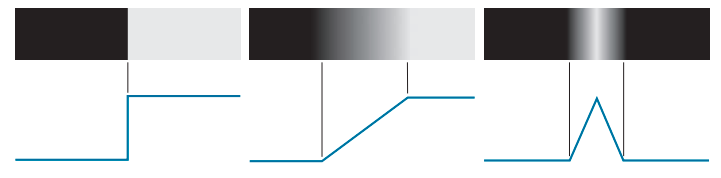
\includegraphics[width=0.9\linewidth]{logoss/intensity.png} % Removed extension
       \caption{Conceptual illustration of intensity gradient at an edge.}
       \label{fig:edge_concept}
     \end{figure}
  \end{block}

   \begin{alertblock}{Important Point}
    \centering
    \textbf{Scan QR code for more details}
    \begin{figure}[h]
        \centering
        
\includegraphics[width = 0.5\textwidth]{logoss/qr.png}
        \label{fig:my_zero}
    \end{figure}
  \end{alertblock}

\end{column} % End Column 1



\separatorcolumn 

% ====================
% Column 2
% ====================
\begin{column}{\colwidth}

  \begin{block}{Mathematical Formulation} \setlength{\parskip}{1pt} \linespread{1.0}

    Let $f(x, y)$ be the image intensity at pixel $(x, y)$. The gradient is approximated by convolving the image with specific kernels.

    \textbf{Gradient Magnitude ($G$)}: Often approximated as:
    \begin{equation*}
        G = \sqrt{G_x^2 + G_y^2} \quad \text{or} \quad G \approx |G_x| + |G_y|
    \end{equation*}
    where $G_x$ and $G_y$ are the responses from the horizontal and vertical kernels, respectively.

    \textbf{Gradient Direction ($\theta$)}:
    \begin{equation*}
        \theta = \operatorname{atan2}(G_y, G_x)
    \end{equation*}

    \textbf{Kernels ($k_x, k_y$):}

    \textit{Roberts Cross Kernels:}
    \begin{equation*}
    k_x = \begin{pmatrix} +1 & 0 \\ 0 & -1 \end{pmatrix} \quad
    k_y = \begin{pmatrix} 0 & +1 \\ -1 & 0 \end{pmatrix}
    \end{equation*}
    Note: Applied centered differently than 3x3, effectively measures diagonal differences.

    \textit{Prewitt Kernels:}
    \begin{equation*}
    k_x = \begin{pmatrix} -1 & 0 & +1 \\ -1 & 0 & +1 \\ -1 & 0 & +1 \end{pmatrix} \quad
    k_y = \begin{pmatrix} -1 & -1 & -1 \\ 0 & 0 & 0 \\ +1 & +1 & +1 \end{pmatrix}
    \end{equation*}

    \textit{Sobel Kernels:}
    \begin{equation*}
    k_x = \begin{pmatrix} -1 & 0 & +1 \\ -2 & 0 & +2 \\ -1 & 0 & +1 \end{pmatrix} \quad
    k_y = \begin{pmatrix} -1 & -2 & -1 \\ 0 & 0 & 0 \\ +1 & +2 & +1 \end{pmatrix}
    \end{equation*}

    \textbf{Convolution Operation:}
    The gradient components are calculated as:
    \begin{equation*}
    G_x = k_x * f(x, y) \quad \text{and} \quad G_y = k_y * f(x, y)
    \end{equation*}
    where $*$ denotes the 2D convolution operation.

    \textbf{Edge Thresholding:}
    After computing the gradient magnitude $G$ for all pixels, a threshold $T$ is applied:
    \begin{equation*}
    \text{Edge Pixel if } G(x, y) > T
    \end{equation*}
    Choosing an appropriate threshold is critical and often requires experimentation or adaptive methods.

  \end{block}

  \begin{block}{Visual Comparison \& Results}

   \textbf{Summary Table:}
    \begin{table}[h!]
    \centering \small
    \begin{tabular}{lccc}
      \toprule
      \textbf{Feature} & \textbf{Roberts} & \textbf{Prewitt} & \textbf{Sobel} \\
      \midrule
      Kernel Size      & 2x2       & 3x3       & 3x3 \\
      Emphasis         & Diagonal  & Uniform   & Center Pixels \\
      Noise Sensitivity& High      & Medium    & Low-Medium \\
      Computational Cost& Very Low  & Low       & Low \\
      Common Use       & Basic Edu & Simple Apps & General Purpose \\
      \bottomrule
    \end{tabular}
    \caption{Comparison of First-Order Edge Detectors.}
    \label{tab:comparison}
    \end{table}
  \end{block}
  
    We applied the three operators to a standard test image. The results highlight their different characteristics.
    % ** IMPORTANT: Ensure these image files (png/jpg/pdf) exist in 'logos' folder **
    \begin{figure}[h!]
  \centering
  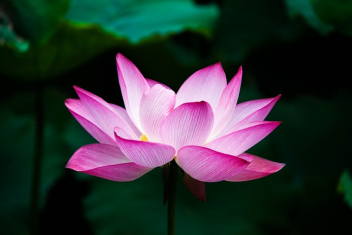
\includegraphics[width=0.47\linewidth]{logoss/original.png}
  \caption{Original Test Image}
  \label{fig:original}
\end{figure}

\begin{figure}[h!]
  \centering
  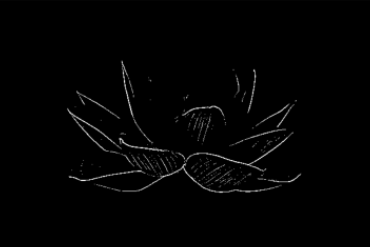
\includegraphics[width=0.47\linewidth]{logoss/robert.png}
  \caption{Roberts Operator Edge Detection}
  \label{fig:roberts}
\end{figure}

\begin{figure}[h!]
  \centering
  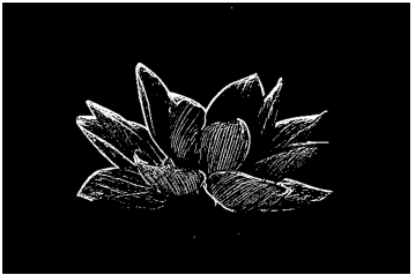
\includegraphics[width=0.47\linewidth]{logoss/Prewitt.png}
  \caption{Prewitt Operator Edge Detection}
  \label{fig:prewitt}
\end{figure}

\begin{figure}[h!]
  \centering
  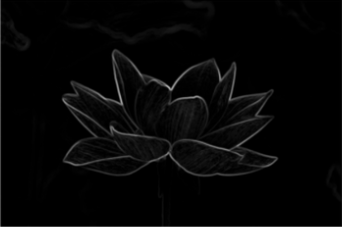
\includegraphics[width=0.47\linewidth]{logoss/sobel.png}
  \caption{Sobel Operator Edge Detection}
  \label{fig:sobel}
\end{figure}

    \textbf{Observations:}
    \begin{itemize}
        \item \textbf{Roberts:} Produces thin edges but is visibly noisy. Misses some horizontal/vertical edges.
        \item \textbf{Prewitt:} Less noisy than Roberts, detects edges more uniformly.
        \item \textbf{Sobel:} Smoothest result, thicker edges, good noise suppression compared to the others. Captures major boundaries well.
    \end{itemize}

   

\end{column} % End Column 2

\separatorcolumn % Right separator

% ====================
% Column 3
% ====================
\begin{column}{\colwidth}

  % Add this to your preamble


\begin{block}{Discussion}
  \begingroup
  \let\oldraggedright\raggedright
  \renewcommand{\raggedright}{\justifying} % Enable justification
  
    \textbf{Advantages:}
    \begin{itemize}
        \item Simplicity and computational efficiency.
        \item Intuitive basis in calculus (approximating derivatives).
        \item Effective for images with strong edges and low noise.
    \end{itemize}

    \textbf{Limitations:}
    \begin{itemize}
        \item \textbf{Noise Sensitivity:} Derivatives amplify noise. Performance degrades significantly in noisy images without pre-smoothing (e.g., Gaussian filtering).
        \item \textbf{Edge Thickness:} Detected edges can be multiple pixels thick, requiring post-processing like non-maximum suppression for thinning.
        \item \textbf{Thresholding Dependence:} Performance is highly dependent on the choice of threshold value.
        \item \textbf{Directionality:} Roberts operator is biased towards diagonal edges. Prewitt and Sobel are better but still limited by fixed kernel directions.
    \end{itemize}

    \textbf{Improvements \& Alternatives:} 
    \begin{itemize}
        \item \textbf{Pre-smoothing:} Applying a Gaussian filter before edge detection (e.g., Gaussian + Sobel) reduces noise sensitivity.
        \item \textbf{Canny Edge Detector:} A multi-stage algorithm incorporating Gaussian smoothing, gradient calculation (often Sobel), non-maximum suppression, and hysteresis thresholding. It is generally considered superior but more complex.
        \item \textbf{Second-Order Derivatives:} Methods like the Laplacian operator or Laplacian of Gaussian (LoG) detect edges at zero-crossings of the second derivative, which can provide better localization but are even more sensitive to noise.
    \end{itemize}
  \endgroup
\end{block}
  \begin{block}{Conclusions}
  
    First-order derivative operators (Roberts, Prewitt, Sobel) are foundational techniques for edge detection in digital images. They offer a simple and fast way to approximate the image gradient and identify areas of sharp intensity change.
    \begin{itemize}
        \item \textbf{Roberts} is the simplest but most noise-prone.
        \item \textbf{Prewitt} offers a slight improvement in noise handling.
        \item \textbf{Sobel} provides a good balance between noise suppression and edge detection, making it a popular choice.
    \end{itemize}
    While effective in certain conditions, their sensitivity to noise and dependence on thresholding often necessitate pre-processing or more advanced techniques like the Canny edge detector for robust performance in real-world applications. Understanding these basic methods is crucial for appreciating the development of more sophisticated edge detection algorithms.
  \end{block}

  \begin{block}{References}
    \begin{thebibliography}{9} 
    \bibitem{gonzalezwoods}
        Gonzalez, R. C., \& Woods, R. E. (2018). \textit{Digital Image Processing} (4th ed.). Pearson.
        \newblock (Chapter 10 discusses edge detection, including these methods). \url{https://www.pearson.com/us/higher-education/program/Gonzalez-Digital-Image-Processing-4th-Edition/PGM1784799.html}

    \bibitem{roberts1963}
        Roberts, L. G. (1963). Machine perception of three-dimensional solids. In J. T. Tippett et al. (Eds.), \textit{Optical and Electro-Optical Information Processing} (pp. 159-197). MIT Press.
        \newblock (Seminal work introducing the Roberts Cross operator). Often cited, original access may be limited.

    \bibitem{prewitt1970}
        Prewitt, J. M. S. (1970). Object enhancement and extraction. In B. S. Lipkin \& A. Rosenfeld (Eds.), \textit{Picture Processing and Psychopictorics} (pp. 75-149). Academic Press.
        \newblock (Introduced the Prewitt operator).

    \bibitem{sobel}
         Sobel, I. (1970). Camera Models and Machine Perception. Stanford University, AIM-21. \url{https://apps.dtic.mil/sti/pdfs/AD0704776.pdf} 
        \newblock (While often cited from a 1968 talk with Feldman, this 1970 paper discusses related concepts and is sometimes cited for the operator). Duda \& Hart (1973) also popularised it.

    \bibitem{canny1986}
        Canny, J. (1986). A Computational Approach to Edge Detection. \textit{IEEE Transactions on Pattern Analysis and Machine Intelligence}, PAMI-8(6), 679-698.
        \newblock (\textit{Reference for a more advanced method}). \url{https://doi.org/10.1109/TPAMI.1986.4767851}

    % New additions
    \bibitem{marrHildreth1980}
        Marr, D., \& Hildreth, E. (1980). Theory of Edge Detection. \textit{Proceedings of the Royal Society of London. Series B, Biological Sciences}, 207(1167), 187-217.
        \newblock (Foundational work on Laplacian of Gaussian (LoG) edge detection). \url{https://doi.org/10.1098/rspb.1980.0020}

    \bibitem{shrivakshan2012}
        Shrivakshan, G. T., \& Chandrasekar, C. (2012). A Comparison of Various Edge Detection Techniques Used in Image Processing. \textit{International Journal of Computer Science Issues}, 9(5), 269-276.
        \newblock (Comparative study of classical edge detectors). \url{https://www.ijcsi.org/papers/IJCSI-9-5-1-269-276.pdf}

    \end{thebibliography}
\end{block}

\end{column} % End Column 3

\separatorcolumn % Right separator

\end{columns} % End columns environment
\end{frame} % End frame

\end{document}